\documentclass{beamer}
%\documentclass[handout]{beamer}

\mode<presentation>{
  \usetheme{Dresden}
  \setbeamercovered{transparent}
}

\mode<handout>{
  \usepackage{pgfpages}
  \pgfpagesuselayout{4 on 1}[a4paper,border shrink=5mm,landscape]
  \setbeamercolor{background canvas}{bg=black!5}
}

\usepackage[english]{babel}
\usepackage[latin1]{inputenc}
%\usepackage{times}
%\usepackage[T1]{fontenc}
\usepackage{tikz}
\usepackage{graphicx}
\usepackage{hyperref}
\hypersetup{colorlinks,linkcolor=,urlcolor=blue}%


\usepackage{colortbl}
\usepackage{color}

%\useoutertheme[subsections=false]{smoothbars} % use smaller ribbon at the top

%\setbeamertemplate{navigation symbols}{} %no nav symbols

\usepackage[absolute,overlay]{textpos}
\newenvironment{reference}[2]{
  \begin{textblock*}{\textwidth}(#1,#2)
      \footnotesize\it\bgroup\color{red!50!black}}{\egroup\end{textblock*}}


\title[Display and Management]{Display and Management of Geomatics Research Data}

\author{Michiel Johan Baird \and
    Timothy Daniel Trewartha \and
   \\  Supervisor: Hussein Suleman}

\date{24 May 2012}

\pgfdeclareimage[height=20pt]{university-logo}{images/uct}
\logo{\pgfuseimage{university-logo}}

%\AtBeginSection[]{
%  \begin{frame}<beamer>{Outline}
%    \tableofcontents[currentsection,currentsubsection]
%  \end{frame}
%}

\begin{document}
\begin{frame}
    \titlepage
\end{frame}

\section{Overview}
\subsection{}
\begin{frame}{Zamani Project}
\begin{columns}
\begin{column}{.65\linewidth}
\begin{itemize}
    \item Started by the UCT Department of Geomatics in 2004
    \item Aims to preserve cultural heritage
    \begin{itemize}
    \item Plans
    \item Laser scans
    \item Photos
    \item Videos
    \end{itemize}
\end{itemize}
\end{column}
\begin{column}{.35\linewidth}
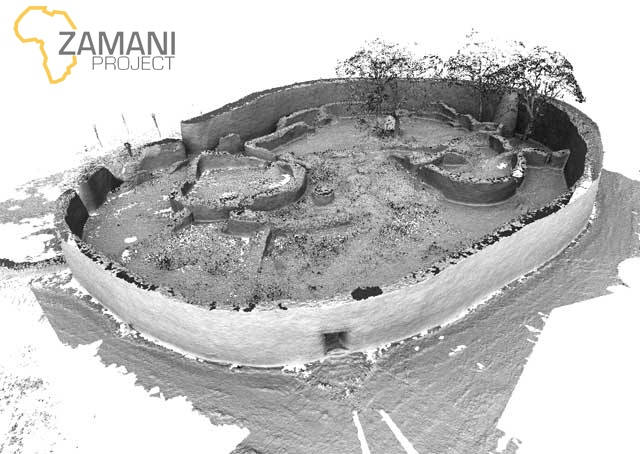
\includegraphics[width=\linewidth]{images/zamani1.jpg} \\
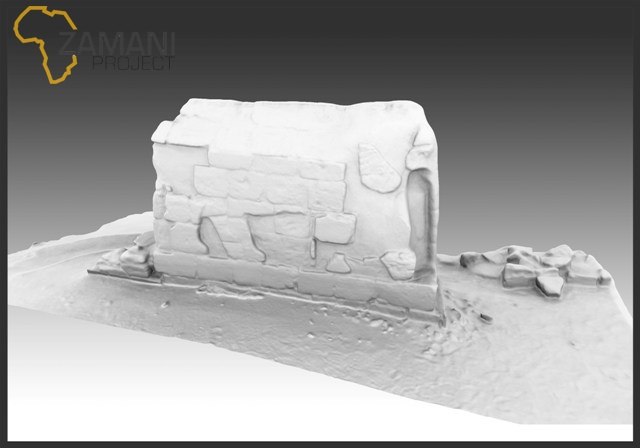
\includegraphics[width=\linewidth]{images/zamani2.jpg}
\end{column}
\end{columns}

\end{frame}

\begin{frame}{Zamani Project}
\begin{columns}
\begin{column}{.65\linewidth}
\begin{itemize}
    \item Over 100 models of sites in various African countries
    \item These models are big
    \item Containing upwards of a billion points
\end{itemize}
\end{column}
\begin{column}{.35\linewidth}
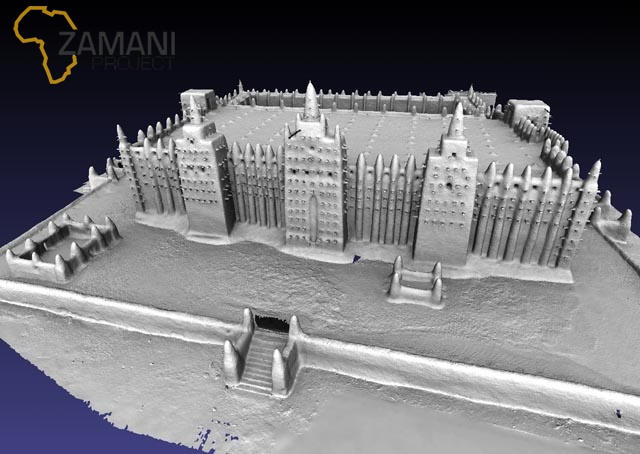
\includegraphics[width=\linewidth]{images/zamani3.jpg} \\
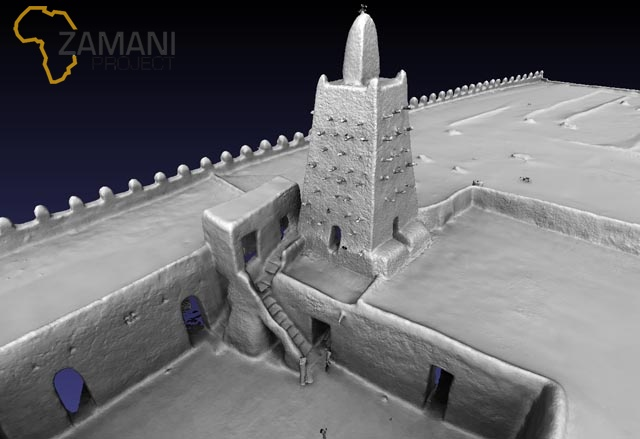
\includegraphics[width=\linewidth]{images/zamani4.jpg}
\end{column}
\end{columns}

\end{frame}

\begin{frame}{Problems Faced}
\begin{itemize}
    \item Fast-growing volume of data
    \item Difficulty in storing the data
    \item Difficulty with viewing the large models in real-time
    \item Data management issues
    \item Data locality issues
\end{itemize}
\end{frame}


\begin{frame}{Problems Approached}
    \begin{itemize}
        \item Difficulty with viewing the large models in real-time
        \item Data management issues
    \end{itemize}
\end{frame}

\begin{frame}{Solution Overview}

\begin{itemize}
\item Enable dynamic high density model streaming
\item Create a GIS workbench that facilitates the research
    \end{itemize}
    \begin{center}
    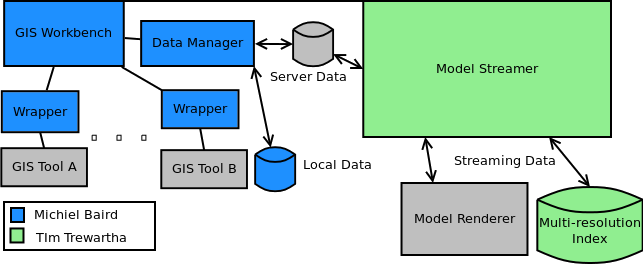
\includegraphics[width=0.8\linewidth]{images/mainDiagram.png}
    \end{center}
\end{frame}

\section{Dynamic Point Cloud Streaming}
\subsection{Tim Trewartha}
\begin{frame}{Dynamic Viewing of Large 3D Models}
\begin{itemize}
\item The Department of Geomatics has indicated that they have difficulties
  handling the sizes of some of their models
\item Some of the models they are dealing with contain over 8 billion points
\item At this point, traditional viewing methods cannot cope; the resolution
  of the original model must be decreased manually beforehand
\item This compromise is often unacceptable
\end{itemize}
\end{frame}


\begin{frame}{Research Question}
\begin{itemize}
\item Is it feasible to support real time viewing of models containing
  billions of points?
\item Answering this question in the affirmative would enable exploration
  of the Zamani models in their full detail
\item It would have a significant impact in the Geomatics department
\end{itemize}
\end{frame}

\begin{frame}{Proposed Solution}

\begin{itemize}
\item Implement a multi-resolution data structure to divide our model into
  manageable chunks
\item Initially only a subset of the points is available
\item As one zooms into the model and greater detail is required, we dynamically
  fetch additional points from our data structure until the full original
  detail is available
\end{itemize}
\end{frame}


\begin{frame}{Relevant Literature}

\begin{itemize}
\item Common approaches to structuring large 3D models include octrees,
  R-trees, bounding sphere hierachies, and Hilbert Space Filling
  Curves
\end{itemize}
{\scriptsize
\begin{tabular}{l|c|l}
 Data Structure & Largest model rendered & Reference \\
\hline
\hline
Bounding Sphere Hierachy  & 8 million points & (Rusinkiewicz and Levoy, 2000) \\
\hline
Hierarchy of Tetrahedra   & 300 million points& (Cigoni et al., 2008)  \\
\hline
Octree          & 2.2 billion points& (Wand et al., 2007)    \\
\end{tabular}}

\end{frame}


\begin{frame}{Proposed DataStructure}

\begin{itemize}
\item From researching the literature it seems that octrees have the best
  performance
\item All data is stored in the leaf nodes
\item Inner nodes provide simplified multi-resolution representations
\item No leaf node should contain more than a specified number of points
\item Empirically, it seems that a value of around 30,000 gives good performance
\end{itemize}
\end{frame}


\begin{frame}{Evaluation Criteria}
\begin{itemize}
\item Can the system render the largest of the Zamani models at interactive
  frame rates?
\item If this goal is achieved the system will be a success
\item Varying degrees of success can also be determined by testing smaller
  models of varying sizes
\end{itemize}
\end{frame}


\section{GIS Workbench}
\subsection{Michiel Baird}
\begin{frame}{Research Question}

\begin{itemize}
\item How effective is an automated workflow solution in GIS context?
\end{itemize}
\end{frame}



\begin{frame}{}
\begin{itemize}
\item Various fields of science has adopted and implemented
  workflow systems
\item These systems have increased efficiency and research output
\item GIS research has been shown to be applicable to an automated
  workflow system; this has not however been implemented
\end{itemize}
\end{frame}


\begin{frame}{Proposed Solution}

\begin{itemize}
\item Use an existing workflow system as various platforms already
  exist
\item Design a workflow that is applicable to GIS
\item Write middleware to integrate with existing GIS tools
\item Software that automatically transfers data as it is needed down
  the pipeline
\end{itemize}
\end{frame}


\begin{frame}{Evaluation Criteria}
\begin{itemize}
\item How much does the content delivery system decrease waiting time?
\item How effective is the workflow system based on the analytics that
  will be generated be the system.
\end{itemize}
\end{frame}


\section{Deliverables and Timeline}
\subsection{}
\begin{frame}{Deliverables}

\begin{itemize}
\item GIS workbench
\item Middleware for core functionalities
\item Data Flow Facilitator
\item Hierarchical Data Structure
\item Streaming Infrastucture
\end{itemize}

\end{frame}

\begin{frame}{Timeline}


{\scriptsize
\begin{tabular}{l|c|l}
Description                      & Start             & End            \\
\hline \hline
Web Presence                     & 25 May            & 12 June        \\
\hline
Initial Feasibilty Demonstration & 11 June           & 29 June        \\
\hline
Background Chapter               & 2 July            & 29 July        \\
\hline
Design Chapter                   & 29 July           & 29 August      \\
\hline
First Implementation             & 1 July            & 29 August      \\
\hline
Final Implementation             & 29 August         & 28 September   \\
\hline
Report Outline Complete          & 28 September      & 10 October     \\
\hline
Report                           & 28 September      & 31 October     \\
\hline
Poster                           & 31 October        & 3 November     \\
\hline
Presentation                     & 11 November       & 18 November    \\
\end{tabular}}

\end{frame}

\end{document}
